\documentclass[a4paper,11pt]{article}
\usepackage[utf8]{inputenc}
\usepackage{tikz}
\usepackage{amsmath} \usepackage{amssymb}
\usepackage{amsfonts}
%\usepackage{amscd}
\usepackage{latexsym} \usepackage{mathrsfs} 

\usepackage{ngerman}
\usepackage{yfonts}
\usepackage{color}
%\usepackage[pdftex]{graphicx}
%\usepackage{pdfpages}
\usepackage{dsfont}
\usepackage{xy}\xyoption{all}
\usepackage{enumitem}


%%%%%%%%
\usepackage{graphicx}
\definecolor{MNTFcol}{RGB}{0,101,97}
\definecolor{dunkelgrau}{rgb}{0.5,0.5,0.5}
\definecolor{hellgrau}{rgb}{0.95,0.95,0.95}
\definecolor{neuePO}{rgb}{0.85,0.85,0.94}
\definecolor{purp4}{rgb}{0.36,0.28,0.55}
\definecolor{silv}{rgb}{0.45,0.45,0.50}
\usepackage{colortbl}


\setlength{\textwidth}{18cm} %% eigentlich 16cm
\setlength{\oddsidemargin}{-10mm} %%eigentlich 0mm
\setlength{\evensidemargin}{0mm}
\setlength{\unitlength}{1mm}
\setlength{\textheight}{22cm}
%\voffset=-3cm

\renewcommand{\familydefault}{\sfdefault}
\usepackage{helvet}

\def\R{{\mathbb R}} \def\C{{\mathbb C}} \def\N{{\mathbb N}}
\def\Z{{\mathbb Z}} \def\Pj{{\mathbb P}} \def\cc{{\cal C}}
\def\Q{{\mathbb Q}} \def\vi{\varphi} \def\ve{\varepsilon}
\def\F{{\mathbb F}}
\newcommand{\cO}{\mathcal{O}}
\newcommand{\cM}{\mathcal{M}}
\newcommand{\cN}{\mathcal{N}}
\newcommand{\cF}{\mathcal{F}}
\newcommand{\cG}{\mathcal{G}}
\newcommand{\cH}{\mathcal{H}}
\newcommand{\cHom}{\mathcal{H}om}
\newcommand{\GL}{\mathrm{GL}}
\newcommand{\Ab}{\mathcal{A}b}

\newcommand{\falle}[1]{\underset{{#1}}{\forall} \ }
\newcommand{\gibts}[1]{\underset{{#1}}{\exists} \ }


\newcommand{\lto}{\longrightarrow}
\newcommand{\widebar}[1]{\overline{#1}}
\newcounter{aufg}
\newcommand{\Aufg}{\stepcounter{aufg}\vspace*{0.2cm}\noindent{\bf
    Aufgabe \arabic{aufg}:} }
\newcommand{\tAufg}{\stepcounter{aufg}\vspace*{0.2cm}\noindent{\bf
    "U.Aufgabe \arabic{aufg}:} }

\newcommand{\sAufg}{\vspace*{0.7cm}\noindent{\bf $\ast $-Aufgabe:} }
\renewcommand{\labelenumi}{{\rm \roman{enumi})}}

\newcommand{\sRHom}{\mathrm{R}\mathcal{H}om}
\newcommand{\Hom}{\text{Hom}}
\newcommand{\cB}{\mathcal{B}}
\newcommand{\cA}{\mathcal{A}}
\newcommand{\cD}{\mathcal{D}}
\newcommand{\cC}{\mathcal{C}}
\newcommand{\cL}{\mathcal{L}}
\newcommand{\eig}[1]{\mathrm{Eigenwerte}(#1)}
\newcommand{\isoto}{\stackrel{\cong}{\lto}}
\newcommand{\companion}[1]{\mathrm{Begleit}(#1)}
\newcommand{\sbt}{\text{\tiny$\bullet$}}
\newcommand{\Kom}{\mathrm{Kom}}

\begin{document}
\sffamily
\setlist[enumerate]{leftmargin=*}

\pagestyle{empty}

\unitlength1mm

\begin{picture}(100,50)

\put(-8,52){
\includegraphics[scale=0.4]{Uni_Aug_Logo_MNTF_RGB}}

\put(110,82){
\begin{minipage}[t]{6cm} \baselineskip10pt
 \rule[2.5mm]{6cm}{.3pt}
 
  {\scriptsize\bf  Prof. Dr. Marco Hien\\
  M. Sc. Thomas Bargen\\
 \rule{6cm}{.3pt}}
\end{minipage}
}
\end{picture}

\vspace*{-6.5cm}
\centerline{\Large Aufgaben zu {\it Riemannsche Flächen} -- WS 2025/26}


\medskip \centerline{3. Blatt}


\setcounter{aufg}{7}
\newcounter{labl}

\vspace*{1cm}
Auf diesem Blatt bezeichnet $\Lambda_\tau:=\mathbb{Z}1\oplus\mathbb{Z}\tau$ stets das Gitter für $\tau \in \mathbb{H} := \{ z \in \mathbb{C} \mid \operatorname{Im}(z) > 0 \}$.

\medskip

\Aufg Seien $\tau \in \mathbb{H}$ gegeben und
\[
\begin{pmatrix}
	a & b \\ c & d
\end{pmatrix} \in SL_2(\mathbb{Z}) = \{ A \in \operatorname{Mat}(2 \times 2, \mathbb{Z}) \mid \det(A) = 1 \}.
\]

Zeige: Wenn $\tau' = \frac{a\tau + b}{c\tau + d}$ gilt, dann sind die beiden Tori $\mathbb{C}/\Lambda_\tau$ und $\mathbb{C}/\Lambda_{\tau'}$ isomorph.

\emph{Hinweis}: Überlege zuerst, warum $\tau'\in\mathbb{H}$ gilt.

\medskip

\Aufg Sei $\alpha : \mathcal{F} \to \mathcal{G}$ ein Morphismus von Garben auf einem topologischen Raum $X$. 
\begin{enumerate}
	\item Begründe, dass $\alpha$ zu jedem $x \in X$ einen Gruppenhomomorphismus $\alpha_x : \mathcal{F}_x \to \mathcal{G}_x$ auf den Halmen induziert.
	\item Zeige: Ist $U \subset X$ offen und $\alpha_x$ für alle $x \in U$ injektiv, so ist auch $\alpha(U) : \mathcal{F}(U) \to \mathcal{G}(U)$ injektiv.
\end{enumerate}

\medskip

\Aufg Auf $\mathbb{CP}^1$ betrachte die beiden offenen Mengen
\[
U_0 := \mathbb{C} \quad \text{und} \quad U_1 := \mathbb{CP}^1 \setminus \{0\}.
\]
Sei $m \in \mathbb{Z}$. 
\begin{enumerate}
	\item Zeige, dass durch die Zuordnung
	\[
	U \mapsto \{ (f_0, f_1) \mid f_j : U \cap U_j \to \mathbb{C} \text{ holomorph mit } \forall z \in U \cap U_0 \cap U_1: f_0(z) = z^{m} f_1(z) \} 
	\]
	eine Garbe auf $\mathbb{CP}^1$ definiert ist (was sind die Restriktionen?). Wir bezeichnen sie mit $\mathcal{O}_{\mathbb{CP}^1}(m)$.
	\item  Bestimme die \textit{globalen Schnitte} $\mathcal{O}_{\mathbb{CP}^1}(m)(\mathbb{CP}^1)$ dieser Garbe in Abhängigkeit von $m$.
\end{enumerate}


\medskip

\Aufg  Wir betrachten in dieser Aufgabe die Weierstraß $\wp$-Funktion, welche wie folgt definiert ist:
\[
\wp(z) := \frac{1}{z^2} + \sum_{\lambda \in \Lambda_\tau \setminus \{0\}} \left( \frac{1}{(z + \lambda)^2} - \frac{1}{\lambda^2} \right)
\]
\begin{enumerate}
	\item[i)]Begründe, dass dies eine meromorphe Funktion auf dem Torus $T := \mathbb{C}/\Lambda_\tau$ definiert.
	
	\item[ii)] Zeige: $\wp$ hat einen Pol der Ordnung 2 bei $z = 0 + \Lambda_\tau \in T$ und muss mindestens eine Nullstelle besitzen.\footnote{Betrachte dazu $\wp$ als doppelt-periodische Funktion auf $\mathbb{C}$ und benutze ein geeignetes Pol-/Nullstellen zählendes Integral.}
\end{enumerate}

\medskip \emph{Hinweis:} Die Lokalisierung der Nullstellen ist nicht trivial:\footnote{vgl: M. Eichler, D. Zagier, \emph{On the Zeros of the Weierstraß} $\wp$\emph{-function}, Math. Ann. 258, 399–407 (1982)} 

\medskip 

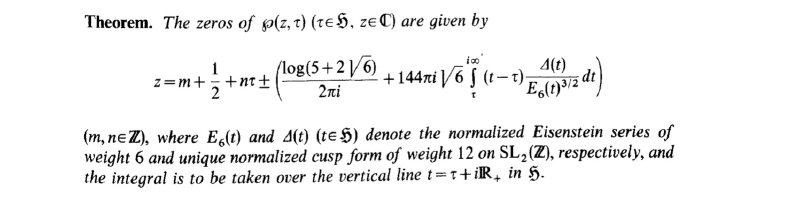
\includegraphics[scale=0.8]{Theorem_ZerosWeierstrass}

\medskip

\end{document}
